\documentclass[12pt,
               color={usenames,   % Since beamer loads color package 
                      dvipsnames},%  automatically \usepackage{color}   
                                  %  cannot be used to pass options.
%               draft,           % Draft WIP version without header &
                                %  footer. Faster compilation.
%               handout,         % Handout version. not sure what it does.
%               notes            % To print notes.
                    ]{beamer}   


%\includeonlyframes{SLIDENOWTWO}    % Use when drafting for fast
                                % compile turnaround time.

\usepackage[normalem]{ulem}

%%%%%%%%%%%%%%%%%%%%%%%%%%%%%%%%%%%%%%%%%%%%%%%%%%%%%%%%%%%%%%%%%%%%%%%%%%%%%
% Theme customization

\usetheme[compress]{Ilmenau}    % Small circle based TOC on top bar
                                %  single line.
%\usetheme[width=1in]{Hannover}  % TOC left side bar.
%\usetheme{Szeged}               % Similar to Ilmenau except borders on
%                                %  top bar and bottom.
%\usecolortheme  {beetle}        % Grey and blue based.
\useinnertheme  {circles}       % Circle dingbats with no shading.
\usefonttheme[onlylarge]
                {structurebold} % Structure fonts are
                                % bold. Set to only the title / big
                                % fonts.
%\useoutertheme[compress,
%               footline=empty]
%               {miniframes}     % Don't use with explicit themes 




% Beamer elements customization: setbeamercolor/-font/-template
% \setbeamercolor{title}                {fg=light3,bg=light1}
% \setbeamercolor{subtitle}             {fg=dark1,bg=light1}
% \setbeamercolor{date}                 {fg=dark1}
% \setbeamercolor{institute}            {fg=dark1}
% \setbeamercolor{frametitle}           {fg=dark1,bg=light1}
% \setbeamercolor{framesubtitle}        {fg=light5}
% \setbeamercolor{structure}            {fg=dark1}
% \setbeamercolor{palette primary}      {fg=light1,bg=light2} % Palette
%                                               % primary, secondary,
%                                               % tertiary, quaternary
%                                               % for headline and
%                                               % footline 
% \setbeamercolor{palette secondary}    {fg=dark2,bg=light3}
% \setbeamercolor{palette tertiary}     {fg=light1,bg=light3} 
% \setbeamercolor{palette quaternary}   {fg=light1,bg=light2} 
% \setbeamercolor{normal text}          {fg=dark2,bg=light1} 
% %\setbeamercolor{block body alerted}   {fg=white} %isn't working
% \setbeamercolor{alerted text}         {fg=white} % contrast}  %light3} 
% \setbeamercolor{block body}           {bg=light5}
% \setbeamercolor{block title}          {fg=light1} %,bg=light3} % Uncomment 
%                                               % for different block
%                                               % heading background




\setbeamertemplate{blocks}[rounded] % Blocks are rounded on the
%                                     % corners
%\setbeamertemplate{blocks}[default] % Blocks are not rounded on the
                                    % corners

\setbeamerfont{framesubtitle}{series={\fontseries{c}}} % Condensed
                                %shape=\sc             % Small caps

%%%%%%%%%%%%%%%%%%%%%%%%%%%%%%%%%%%%%%%%%%%%%%%%%%%%%%%%%%%%%%%%%%%%%%%%%%%%%
% Packages used
\usepackage{setspace}
\usepackage{latexsym}
\usepackage{amssymb}
\usepackage{amsfonts}
\usepackage{amsmath}
%\usepackage{epsfig}
%\usepackage{graphicx}
%\usepackage{epstopdf}
\usepackage{algorithm}
\usepackage{algorithmic}
\usepackage{enumerate}
\usepackage[normalem]{ulem}  % Underline. normalem keeps the default
                             % \em to be italics. 
\usepackage{textcomp}
%\usepackage{pifont}
%\usepackage{natbib}
\usepackage[inline] {./lib/trackchanges}
           %[finalnew]
\addeditor{x}
\addeditor{a}

%%%%%%%%%%%%%%%%%%%%%%%%%%%%%%%%%%%%%%%%%%%%%%%%%%%%%%%%%%%%%%%%%%%%%%%%%%%%%
% Loading spcial fonts
\DeclareMathAlphabet{\mathpzc}{OT1}{pzc}{m}{it}
\DeclareMathAlphabet{\mathcalligra}{T1}{calligra}{m}{n}


%%%%%%%%%%%%%%%%%%%%%%%%%%%%%%%%%%%%%%%%%%%%%%%%%%%%%%%%%%%%%%%%%%%%%%%%%%%%%
% Color definitions

%% Inspired by Kuler - Vintage Beach Wear -
%% http://kuler.adobe.com/#themeID/1507195 
\definecolor{dark1}      {HTML}{8A866A}   % Goldish gray     
                                          %     [Structure, Block heading]
\definecolor{light1}     {HTML}{FFF0C2}   % Pale amber          
                                          %     [Slide BG] 
\definecolor{light2}     {HTML}{9C968B}     % Gambogeish gray [???]
\definecolor{light3}     {HTML}{A36D5C}   % Grayish vermilion   
                                          %     [Title, Header & footer BG] 
\definecolor{dark2}      {HTML}{473C35}   % Dark grayish tangelo
                                          %     [Slide normal text FG]
\definecolor{light5}     {HTML}{A8A87D}   % Greyish olive
                                          %     [Block BG]
\definecolor{contrast}   {HTML}{197DE5}   % Brilliant azure     
                                          %     [Stark Contrast]



%%%%%%%%%%%%%%%%%%%%%%%%%%%%%%%%%%%%%%%%%%%%%%%%%%%%%%%%%%%%%%%%%%%%%%%%%%%%%
% String defs
\def\cA{{\cal A}}  \def\cB{{\cal B}}  \def\cC{{\cal C}}  \def\cD{{\cal D}}
\def\cE{{\cal E}}  \def\cF{{\cal F}}  \def\cG{{\cal G}}  \def\cH{{\cal H}}
\def\cI{{\cal I}}  \def\cJ{{\cal J}}  \def\cK{{\cal K}}  \def\cL{{\cal L}}
\def\cM{{\cal M}}  \def\cN{{\cal N}}  \def\cO{{\cal O}}  \def\cP{{\cal P}}  
\def\cQ{{\cal Q}}  \def\cR{{\cal R}}  \def\cS{{\cal S}}  \def\cT{{\cal T}}  
\def\cU{{\cal U}}  \def\cV{{\cal V}}  \def\cW{{\cal W}}  \def\cX{{\cal X}}
\def\cY{{\cal Y}}  \def\cZ{{\cal Z}}  \def\hA{{\hat A}}  \def\hB{{\hat B}}
\def\hC{{\hat C}}  \def\hD{{\hat D}}  \def\hE{{\hat E}}  \def\hF{{\hat F}}
\def\hG{{\hat G}}  \def\hH{{\hat H}}  \def\hI{{\hat I}}  \def\hJ{{\hat J}}
\def\hK{{\hat K}}  \def\hL{{\hat L}}  \def\hP{{\hat P}}  \def\hQ{{\hat Q}}
\def\hR{{\hat R}}  \def\hS{{\hat S}}  \def\hT{{\hat T}}  \def\hX{{\hat X}}
\def\hY{{\hat Y}}  \def\hZ{{\hat Z}}
\def\A{{\mathcal A}}  \def\bI {\mathbb I}
\def\C{{\mathcal C}}  \def\bO {\mathbb O}
\def\F{{\mathcal F}}  \def\cl {\mathpzc{l}}
\def\H{{\mathcal H}}  \def\cg {\mathpzc{g}}
                      \def\ccT{\mathpzc{T}}

\def\overlap   {\between}
\def\eps       {\epsilon}
\def\icppl     {\maltese} 
\def\invb      {\textreferencemark}
\def\assign    {\leftarrow}

\def\lndisplay      {1}
\def\commentboxsize {7cm}
\def\prelimspace    {2mm}
\def\alertseccolor {contrast}

% For BibTeX formatting \newblock
\def\newblock{\hskip .11em plus .33em minus .07em}
% for Natbib
%\bibpunct{(}{)}{;}{a}{,}{,}


%%%%%%%%%%%%%%%%%%%%%%%%%%%%%%%%%%%%%%%%%%%%%%%%%%%%%%%%%%%%%%%%%%%%%%%%%%%%%
% New/renew commands
% Format of comments in algorithmic package
\renewcommand{\algorithmiccomment}[1]
{ 
  \vspace {0.5mm}
  \hfill
  {\small
  \begin{tabular}{|r}
    \parbox[right]{\commentboxsize}{ \space \tt{ #1 }}\\  
    % {\tt /* #1 */} \hspace{2mm}
  \end{tabular}
  }
}


% % Theorems etc. 
% \newtheorem{observation}{Observation}
\newcommand{\seq}[1]{\left\langle #1 \right\rangle}
\newcommand{\set}[1]{\left\{ #1\right\}}
\newcommand{\supp}[1]{supp\left( #1 \right)}

\def \probdefwidth {0.85\linewidth}
%params: title, input. body: question.
\newenvironment{problemdef}[2]%
{% Begin def.
  \small%
    \par
    \begin{minipage}[b]{\probdefwidth}%{5in}%
%      \vspace{2mm}%
      {\large #1}\\%     Title
%      \hrule
      \begin{tabular}[t]{l|l}%
%        \hline\\
        {\tt Input} & 
        \begin{minipage}[t]{\probdefwidth}%
          #2\\%          Input
        \end{minipage}\\

        {\tt Question} &
        \begin{minipage}[t]{\probdefwidth}%
        %                Type out question
}%
{% End def.
        \end{minipage}\\
      \end{tabular}%
    \end{minipage}\\  
}



%%%%%%%%%%%%%%%%%%%%%%%%%%%%%%%%%%%%%%%%%%%%%%%%%%%%%%%%%%%%%%%%%%%%%%%%%%%%%
% Title slide details
\title[{\bf tree path labeling} -- a generalization of consecutive
       ones property]
         {Tree Path Labeling of Path Hypergraphs}
\subtitle{Generalization of the Consecutive-ones Property}

\author[anju s $|$ \tt{anjuzabil@gmail.com}]{Anju Srinivasan}

\institute[CS09S012]
         {as part of {\bf M.\;S.} by Research \\ 
          advised by {\bf Dr.\;N.\;S.\;Narayanaswamy}\\ 
          CSE, IITM, Chennai - 36}

\date{25 March 2013}


%%%%%%%%%%%%%%%%%%%%%%%%%%%%%%%%%%%%%%%%%%%%%%%%%%%%%%%%%%%%%%%%%%%%%%%%%%%%%
% Document begins

\begin{document}

\frame{
  \titlepage
}

%\section*{Outline}
\frame[label=SLIDENOW]{
  \tableofcontents % [pausesections]
}


\section{Introduction}
\subsection{An Illustration}

\frame{
  \frametitle{An Illustration}

  \begin{centering}
  \begin{itemize}
    \item To introduce the combinatorial problem of TPL.
  \end{itemize}
    
  \end{centering}
}

\frame{
  \frametitle{Study Group Accommodation problem}
% \begin{centering}
  \begin{itemize}[<uncover@+->]
  \item A set of \textbf{$n$ students} arrive for a summer course, say
    $\{a,b,c,d,e,f,g,h,i,j,k\}$, $n= 11$.
  \item They form \textbf{$m$ study groups}, say $\{\textcolor{red}{R},
    \textcolor{blue}{B}, \textcolor{orange}{O},
    \textcolor{green}{G}\}$, $m = 4$
  \item A student may be in more than one study group but {\em will} be in
    at least one, say\\
%     \begin{itemize}
%     \item 
      $\textcolor{red}{R = \{g, h, i, j, k\}}$,
      $\textcolor{blue}{B = \{a, b, e, g\}}$, 
      $\textcolor{orange}{O = \{c, b, d\}}$,
      $\textcolor{green}{G = \{e, f , g, i\}}$
%    \end{itemize}
    
  \item There are $n$ single occupancy \textbf{apartments} in the university campus for their accommodation.
  \item All these apartments are placed such that streets connecting
    them do not form loops - \textbf{streets form a tree}
  \end{itemize}

  \note{}  
%  \end{centering}
}

\frame{
  \frametitle{Study Group Accommodation problem}
% \begin{centering}
  \begin{block}{The problem}
    How should the students be allocated apartments such that:
    \begin{itemize}[<uncover@+->]
    \item {students of each study group are neighbours?}
    \item {i.e. a study group forms \textbf{a path in the tree}.}
    \end{itemize}
 \end{block}
%  \end{centering}
}


\frame{
  \frametitle{Study Group Accommodation problem}
% \begin{centering}
  \begin{tabular}[h]{cc}
   \only<1>{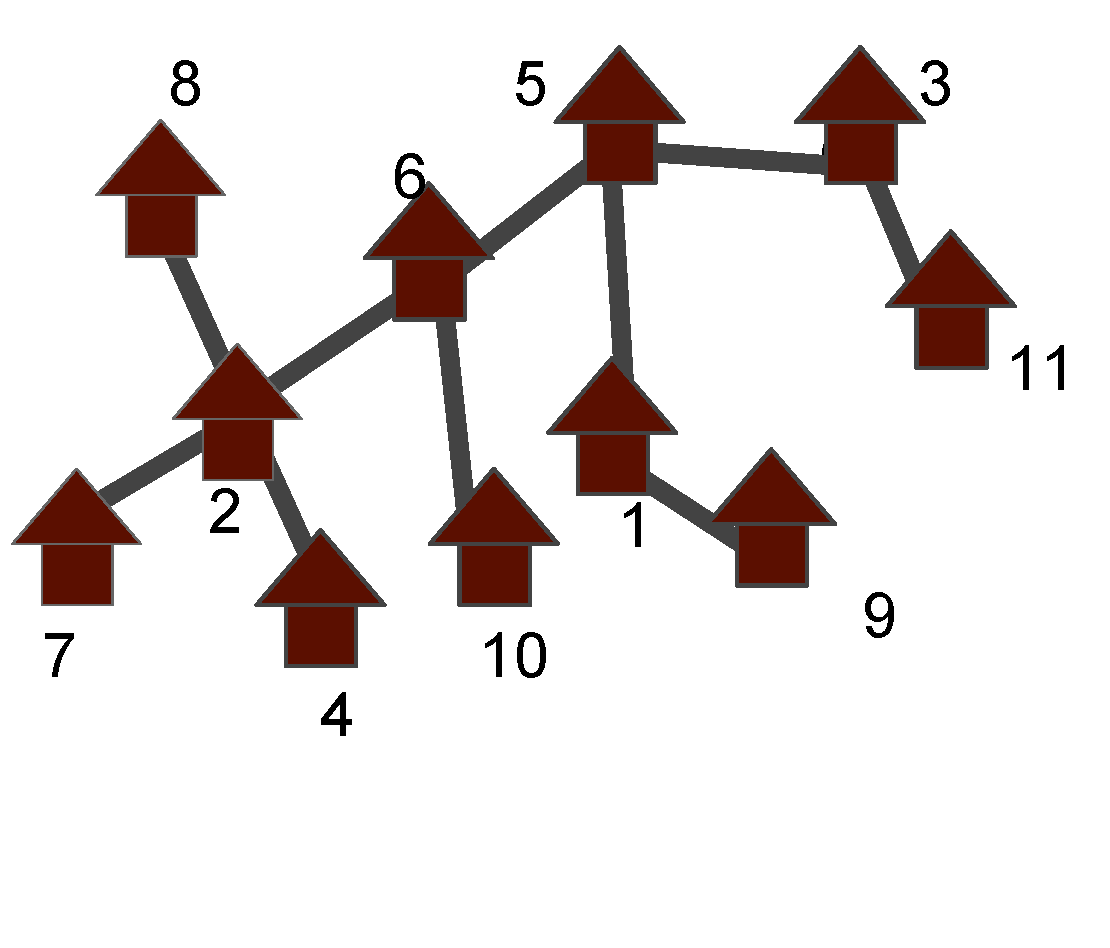
\includegraphics[scale=0.4]{a1.pdf}}
   \only<2>{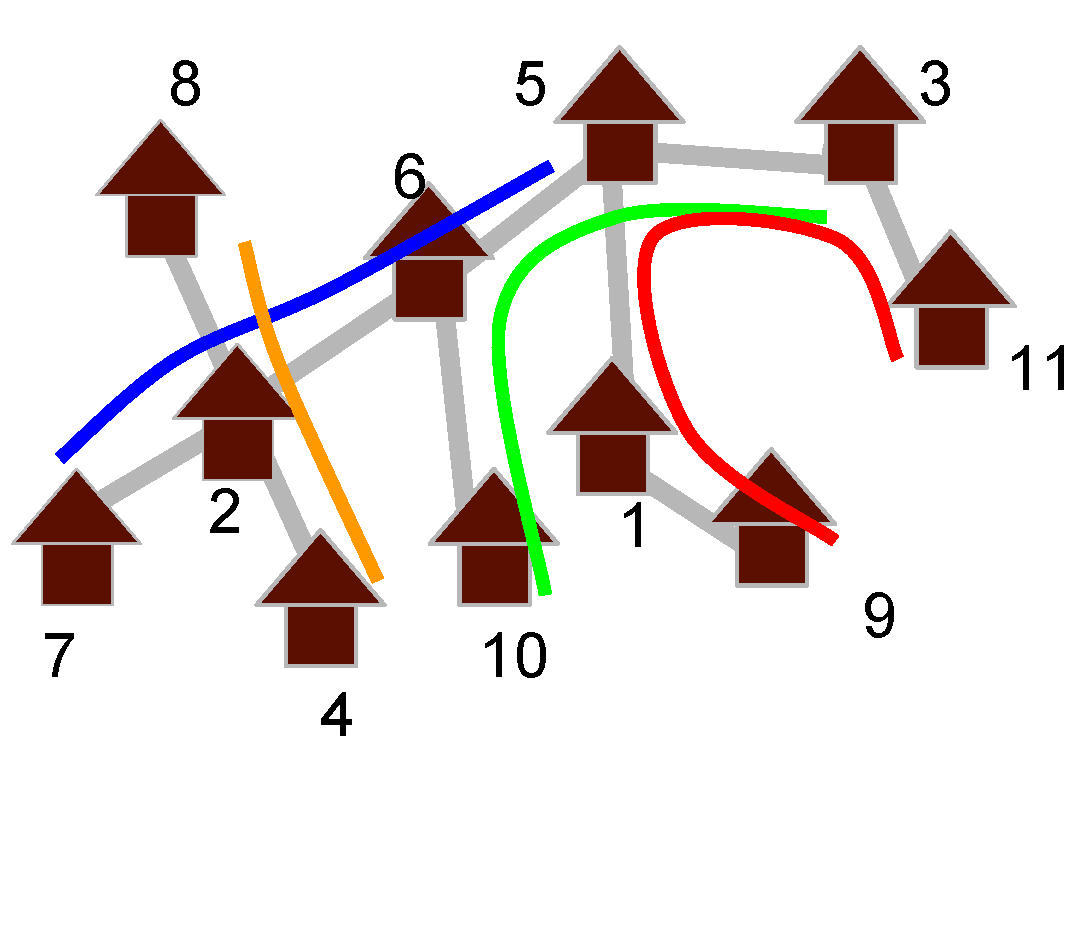
\includegraphics[scale=0.4]{a2.pdf}}
   \only<3>{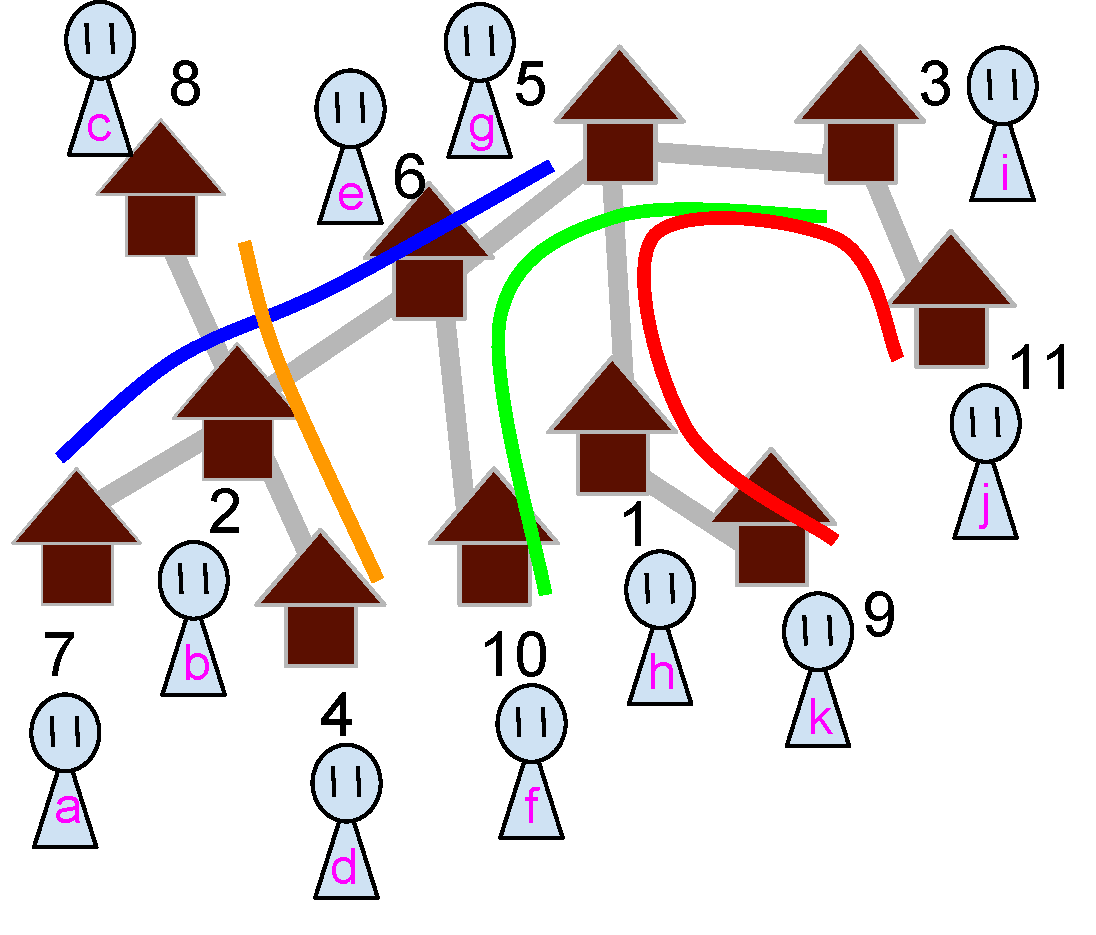
\includegraphics[scale=0.4]{a3_new.pdf}}&
    \parbox[b]{3cm}{
    $\textcolor{red}{R = \{g, h, i, j, k\}}$
      \only<2-3>{ $\textcolor{red}{\rightarrow \{9, 1, 5, 3, 11\}}$}\\
    $\textcolor{blue}{B = \{a, b, e, g\}}$
      \only<2-3>{ $\textcolor{blue}{\rightarrow \{7, 2, 6, 5\}}$}\\
    $\textcolor{orange}{O = \{c, b, d\}}$
      \only<2-3>{ $\textcolor{orange}{\rightarrow \{4, 2, 8\}}$}\\
    $\textcolor{green}{G = \{e, f , g, i\}}$
      \only<2-3>{ $\textcolor{green}{\rightarrow \{10, 6, 5, 3\}}$}
    }
  \end{tabular}
  % \end{centering}
}


\subsection{Terminology}

\frame{ \frametitle{Tree Path Labeling of Path Hypergraphs}
%  \framesubtitle{The combinatorial problem terminology}

  \begin{block}{}
    \begin{itemize}[<uncover@+->]
    \item The set of study groups $\rightarrow$
      \alert{\bf Set system / Hypergraph}
    \item The streets with apartments $\rightarrow$ \alert{\bf
        Target tree}
    \item The path mapping to study groups $\rightarrow$
      \alert{\bf Tree Path Labeling (TPL)}
    \item The apartment allocation $\rightarrow$ \alert{\bf Path
        Hypergraph Isomorphism}
    \end{itemize}
  \end{block}
}

\def\overlayht{4cm}

\frame<1-6>{
  \frametitle{Tree Path Labeling of Path Hypergraphs}

  \begin{block}{}
    \begin{overlayarea}{\textwidth}{\overlayht} 
      \only<1>{There {\em exists} an apartment allocation that
          ``fits'' the path mapping }
      \only<2->{There {\em exists} a
          \alert<2->{hypergraph isomorphism} that ``fits'' the
          \alert<2->{TPL}\\}
      \only<3->{$\Rightarrow$ the TPL is \alert<3->{\sc feasible}\\}

      \only<4->{There {\em exists} \only<4>{an apartment
          allocation}\only<5->{\alert<5-> {a hypergraph isomorphism}} that
          gives \only<4>{some study group path mapping}
      \only<5->{\alert<5->{at least one feasible TPL}\\}} 
      \only<6->{$\Rightarrow$ the hypergraph is a \alert<6->{\sc
       path hypergraph}}
      \end{overlayarea}
  \end{block}

}

\subsection{Motivation}
\frame{
  \frametitle{Consecutive Ones $\rightarrow$ Path Labeling}
  \framesubtitle{The motivation}

   \only<1>{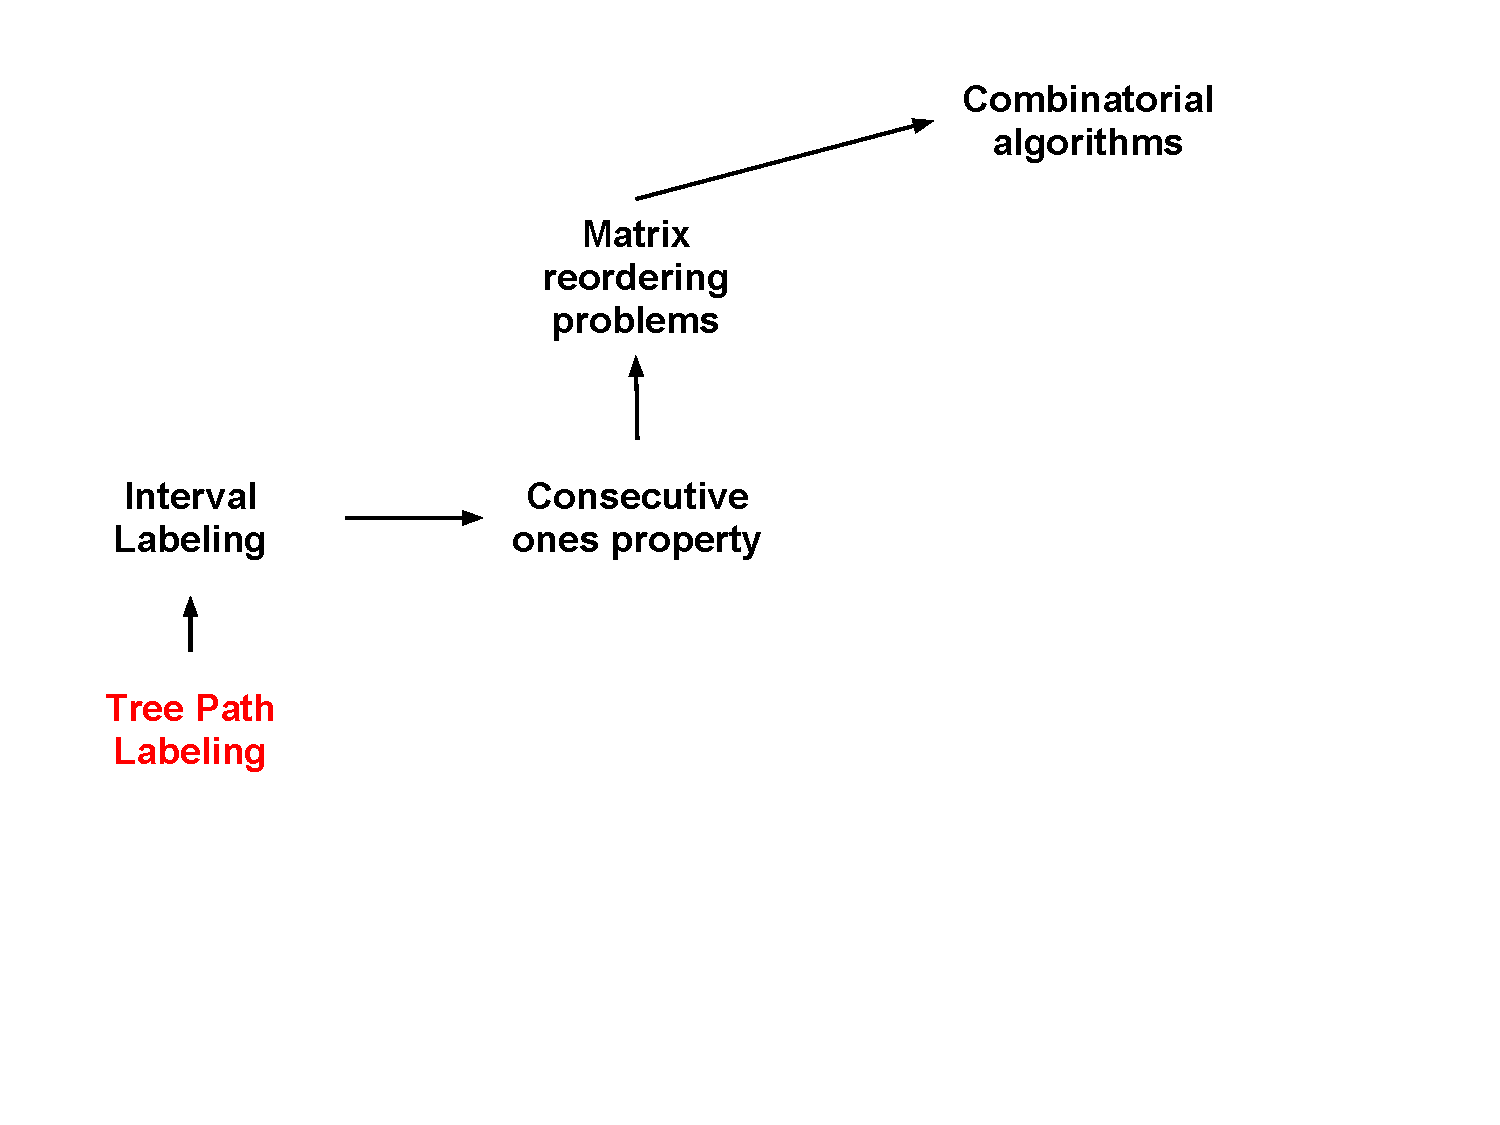
\includegraphics[scale=0.4]{m1.pdf}} 
  
  \tnote[a]{break it down into overlays}
  \note{}
}

% \subsection{Definitions}

% \frame{
%   \frametitle{Tree path labeling of path hypergraphs}
%   \framesubtitle{The two problems}
  
%   \note<1>{}
  
%   \begin{block}{1}
%     {\alert<2>{Characterization} of a {\em feasible TPL} and finding
%       the certificate for feasibility i.e. {\em hypergraph
%         isomorphism}}
%   \end{block}
%   \note[item]<2>{Characterization -- hypergraph + target tree + TPL\\ 
%       (1) is it feasible? \\
%       (2)what is the isomorphism?}

%   \begin{block}{2}
%     {\alert<2>{Computation} of a {\em feasible TPL} if any}
%   \end{block}
%   \note[item]<2>{Computation -- hypergraph + target tree\\ 
%       (1) does there exist a
%       feasible TPL?

%   }
% }

% \frame<1>[label=intro:q1]{
% %\frame<1,9>[label=intro:q1]{
% % 1   : display normal
% % 9   : TBD defined prelim
% % 2-7 : each TBD definition highlight
% % 8   : misc definition highlight
%   \begin{center}
%     {\Huge 1}
%   \end{center}
%     \begin{block}{Characterization of feasible TPL}
%     Given
%     \begin{enumerate}[i. ]
%     \item a \textcolor<9>{\alertseccolor}
%            {\alert<2>{set system or hypergraph}} $\cF$,
%     \item a \textcolor<9>{\alertseccolor}
%            {\alert<3>{feasible} \alert<4>{TPL}} $\cl:\cF \rightarrow
%       \cP$ where $\cP$ is a path system from tree $T$ and $
%       \textcolor<9>{\alertseccolor}{\alert<5,2>{supp(} \cP \alert<5,2>{)}} = V(T)$,
%     \end{enumerate}
%     \uline{what is the \textcolor<9>{\alertseccolor}{\alert<6>{hypergraph
%         isomorphism}}} \[\underline{\phi: \supp{\cF} \rightarrow
%       \supp{\cP}}\] \uline{such that the
%       \textcolor<9>{\alertseccolor}{\alert<7,4>{induced labeling}}} 
%     $\underline{\cl_\phi = \cl}$?
%   \end{block}

%   \note[item]<1>{}
%   \note[item]<9>{to understand this these will be defined in the
%     following slides}
%   \note[item]<2>{first we'll see what a set system or hypergraph is}
%   \note[item]<6>{Next is hypergraph iso}
%   \note[item]<4>{tree path labeling}
%   \note[item]<3>{feasibility of TPL}
% }

% % \againframe<2>{intro:q1}

% % \frame<1-3>{
% %   \frametitle{}
% %   \begin{definition}[Set system, Support of set system] 
% %    The set $\F \subseteq (2^{U} \setminus
% % \emptyset)$ is a \alert {set system} of a universe $U$ with $|U| = n$.\\

% %    The \alert {support of a set system} $\F$ is
% %     the union of all the sets in $\F$.\\ 
% %    $ \ \ \ \ \ \ \ \ \ \ \ \ \ \ \alert{supp(\F) = \bigcup_{S \in \F}S}$
% %   \end{definition}

% %   \note[item]<1>{}

% %   \begin{definition}<2->[Hypergraph] 
% %   A \alert{hypergraph} is exactly same as a graph except that an
% %   ``edge'' can have more than two
% %   vertices and are called \alert{hyperedges}.
% %   \end{definition}

% %   \note[item]<2>{}

% % %  \begin{block}<3>{} 
% % %   $\cF$ can be \alert<3>{ visualized as a
% % %       hypergraph} -- \alert<3>{ vertex set is $supp(\cF)$}, \alert<3>{ hyperedges are the sets
% % %       in $\cF$.}
% % % \end{block}

% %   \only<3>{ 
% %   $\cF$ can be \textbf{visualized as a
% %       hypergraph} -- \textbf{vertex set is $supp(\cF)$},
% %     \textbf{hyperedges are the sets 
% %       in $\cF$.}
% %    }

% %   \note[item]<3>{}

% % %   \begin{block}{Definition}
    
% % %   \end{block}
% % }

% % \againframe<6>{intro:q1}

% % \frame{
% %   % \frametitle{}
% %   \begin{definition}<1->[Hypergraph isomorphism \cite{kklv10}]
  
% %     Two hypergraphs $\cF'$, $\cF''$ are said to be isomorphic,
% %       \alert{ $\cF' \cong \cF''$}

% %   $\ \ \ \ \ \ \ \ \ \ \ \ \ \ \ \ \ \ \ \ \ \ \ \ \ \ \ \ \ \ \ \ \ \
% %   \Longleftrightarrow$        
 
% %   there \alert{ exists a 
% %     bijection $\phi: supp(\cF') \rightarrow supp(\cF'')$} s.t. \\

% %     \alert{   for
% %     all sets $A \subseteq supp(\cF')$
% % $A \in \cF'$ $\Leftrightarrow$
% %     $B \in \cF''$ where $B = \{\phi(x) \mid x \in
% %     A\}$}, written as $B=\phi(A)$.
% %   \end{definition}
% % }

% % \againframe<4>{intro:q1}

% % \frame{
% % %  \frametitle{Tree path labeling (TPL)}

% %   \begin{overlayarea}{\textwidth}{5cm}
% %   \begin{definition}<1->[Tree Path Labeling (TPL)]
% %     For a set system $\cF$, \alert{$\cl: supp(\cF) \rightarrow \cP$} where
% %     $\cP$ is a set of paths from $T$, is called a \alert{TPL} if their
% %     intersection graphs are isomorphic \textcolor<2->{contrast}{(not
% %       hypergraph isomorphism)} \alert{$\bI(\cF) \cong \bI(\cP)$},
% %     $\cl$ is the isomorphism.\\
 
% %    Alternate notation for the \alert{path representation} $\cP$ is \alert{$\cF^\cl$}.
% %   \end{definition}
% %   \only<2>{i.e. intersection properties are preserved. but {\bf not}
% %     necessarily intersection cardinality properties.}
% %   \end{overlayarea}
% %   \begin{definition}<3->[Induced TPL]
% %    If $\cF \cong \cP$ \textcolor<4>{contrast}{(hypergraph
% %      isomorphism)} and $\phi$ is the isomorphism $\Longrightarrow$
% %    this induces a path labeling. This is called \alert{induced path
% %      labeling, $\cl_\phi$}
    
% %   \end{definition}

% % }

% % \againframe<3>{intro:q1}

% % \frame{
% % %  \frametitle{Feasible labeling}

% %   \begin{definition} [Feasible TPL]
% %     A TPL $(\cF, \cl)$ is defined to be \alert{feasible} if
% % % $\cF \cong \cF^\cl$ and this
% % there is \alert{a hypergraph isomorphism $\phi: supp(\cF) \rightarrow
% % supp(\cF^\cl)$} $=V(T)$ which induces path labeling $\cl_\phi: \cF \rightarrow
% % \cF^\cl$ such that \alert{$\cl_\phi = \cl$}.
% %   \end{definition}

% %   \only<2->{ Recall:
% %     \begin{itemize}
% %     \item<2-> $\cF \cong \cF^\cl$ and $\phi$ is the \textbf{hypergraph
% %         isomorphism}
% %     \item<3-> $\bI(\cF) \cong \bI(\cF^\cl)$ and $\cl$ is the \textbf
% %       {graph isomorphism}
% %     \item<4-> \textbf{and} the induced TPL $\cl_\phi$ must be same as $\cl$.
% %     \item<5-> If there is such a $\phi$ then $\cl$ is feasible.
% %     \end{itemize}
% %   }

% % }

\def \TPL {TPL }
\def \ICPPL {ICPPL }
\def \FTPL {\textsc{Feasible Tree Path Labeling} }
\def \CFTPL {\textsc{Compute Feasible Tree Path Labeling} } 
\def \kstar {$k$-subdivided star }
\def \kstars {$k$-subdivided stars }
\def \CFTPLINT {\textsc{Compute Interval
    Labeling} } 
\def \CFTPLKTREE {\textsc{Compute $k$-subdivided Star Path
    Labeling} } 

\section{Problems}

\frame<1-2>[label=intro:q1]{
  \begin{block}{\sc \CFTPL}
    \begin{overlayarea}{\textwidth}{\overlayht} 
    \only<1>
    {
      \begin{problemdef}{\ }{A hypergraph $\cF$ with vertex set $U$
          and a tree $T$.}
        Does there exist a set of paths $\cP$ from $T$ and a bijection
        $\cl$~$:$~$\cF \rightarrow \cP$, such that {\FTPL} returns
        {\bf true} on $(\cF, T, \cl)$.
      \end{problemdef}
    }
    \only<2>
    {
      \begin{itemize}
      \item Is the given hypergraph $\cF$ a \alert{path hypergraph} w.r.t. target tree $T$?
      \item i.e. find at least one feasible tree path labeling $\cl:
        \cF \rightarrow P$, $P$ is a set of paths on $T$.
      \item Complexity is inconclusive for arbitrary trees,
        polynomial time for certain classes of trees.
      \end{itemize}
    }
  \end{overlayarea}
\end{block}
  \note{}% 
}

\def\overlayht{4.5cm}
\frame<1-2>[label=intro:q2]{
  \begin{block}{\sc \FTPL}
    \begin{overlayarea}{\textwidth}{\overlayht} 
    \only<1> {
      \begin{problemdef}{\ }{A hypergraph $\cF$ with vertex set $U$, a
          tree $T$, a set of paths $\cP$ from $T$ and a bijection
          $\cl$~$:$~$\cF \rightarrow \cP$.}

        Does there exist a bijection $\phi$~$:$~$U \rightarrow V(T)$
        such that $\phi$ when applied on any hyperedge in $\cF$ will
        give
        the path mapped to it by the given tree path labeling $\cl$.\\
        { i.e., $\cl(S) = \{\phi(x) \mid x \in S\}$, for every
          hyperedge $S \in \cF$.}
      \end{problemdef}
    }
    \only<2>
    {
      \begin{itemize}
      \item Is the given TPL $\cl$ of hypergraph $\cF$ on tree $T$ feasible?
      \item What is the \alert{hypergraph isomorphism} $\phi: U \rightarrow V(T)$?
      \item Solvable in polynomial time.
      \end{itemize}
      
    }
  \end{overlayarea}
\end{block}
  \note{}% 
}

\def\overlayht{3.5cm}
\frame<1-2>[label=intro:q3]{
  \begin{block}{\sc \CFTPLINT}
    \begin{overlayarea}{\textwidth}{\overlayht} 
    \only<1>{\CFTPL when target tree is an \alert{interval or path $P_n$}}
    \only<2> 
    {
      \begin{itemize}
      \item Is the given hypergraph $\cF$ an \alert{interval
          hypergraph} \cite{kklv10}?
      \item Equivalent to consecutive ones property checking or ICPIA \cite{nsnrs09}
      \item Solvable in polynomial time.
      \end{itemize}      
    }
    \end{overlayarea}
  \end{block}
  
  \note{}% 
}

\def\overlayht{4cm}
\frame<1-2>[label=intro:q4]{
  \begin{block}{\sc \CFTPLKTREE}
    \begin{overlayarea}{\textwidth}{\overlayht}
      \only<1>{ \CFTPL when target tree is a \alert{\kstar} and every
        hyperedge in $\cF$ is of \alert{size at most $k+2$}} \only<2>
      {
        \begin{itemize}
        \item Solvable in polynomial time.
        \end{itemize}
      }
    \end{overlayarea}
  \end{block}
  
  \note{}%
}


\def\overlayht{8cm} 
\frame { %
  \frametitle{$k$-subdivided star}%
  \begin{overlayarea}{\textwidth}{\overlayht}
    \begin{block}{}
      A star with all its edges subdivided exactly $k$ times.
    \end{block}

%  \begin{tabular}[b]{lr}
    \only<2>{ 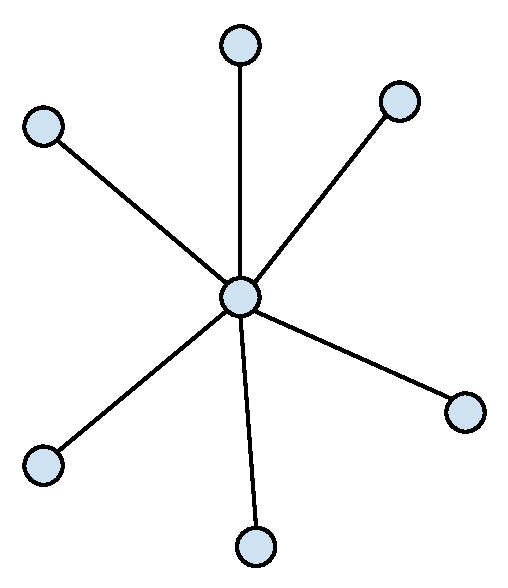
\includegraphics[scale=0.5]{star.pdf} $k = 0$, star }
    \only<3->{ 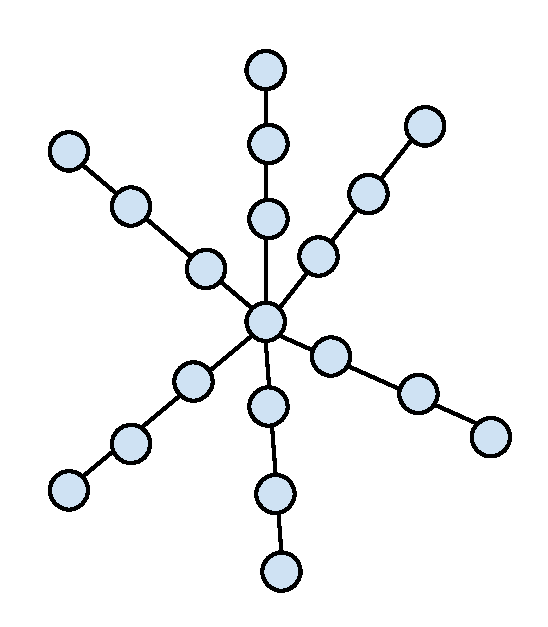
\includegraphics[scale=0.5]{kstar.pdf} 2-subdivided star}
%  \end{tabular}
  
 \end{overlayarea}
}

% %\againframe<1>{intro:q2}


\section[Characterization]{Characterization of a feasible TPL}
\def\overlayht{4cm}
%\frame[label=SLIDENOW] {
\againframe<1>{intro:q2}
%}


\subsection{ICPPL}
\frame [label=SLIDENOW] { % [label=icppl:pr]{ %
  \frametitle{A characterization of feasible TPL}
%  \begin{overlayarea}{\textwidth}{\overlayht}
    \begin{block}<1->{Intersection Cardinality Preserving Path Labeling (ICPPL)}
      A path labeling $(\cF, \cl)$ on the given tree $T$ s.t.
      \[|S_1 \cap S_2 \cap S_3| = |\cl(S_1) \cap \cl(S_2) \cap
      \cl(S_3)|\]
      for all not necessarily distinct $S_1, S_2, S_3 \in
      \cF$

    \end{block}
%\end{overlayarea}
  
\begin{theorem}<2->
  \label{th:charac}
  A path labeling $(\cF, \cl)$ on tree $T$ is feasible iff it is an
  ICPPL.
\end{theorem}


  \note{}
}

\def \filteri {{\tt filter common leaf} }
\def \filterii {{\tt filter fix leaf} }


\frame [label=SLIDENOW]{ % [label=th:icpplth]{ % 
  \frametitle{Finding path hypergraph isomorphism $\phi$}
  \framesubtitle{Given an ICPPL $(\cF, \cl)$ on tree $T$}
  \begin{block}{}
    \begin{itemize}[<uncover@+->]
    \item Uses two filters to refine $(\cF,\cl)$
    \item \alert{\filteri} - ensures that the resulting ICPPL has no two path labels
      sharing a leaf.
    \item \alert{\filterii} - finds the pre-image of each leaf in $T$.
    \item Remove leaves from $T$  and their preimages from $\cF$. Repeat
      filters until $T$ becomes a path.
    \item When $T$ is a path, problem becomes interval assignment. Use
      ICPIA \cite{nsnrs09}
    \end{itemize}
  \end{block}
  

  \note{}
}

\frame [label=SLIDENOW]{ % [label=th:icpplth]{ % 
  \frametitle{Finding path hypergraph isomorphism $\phi$}
  \framesubtitle{\filteri $(\cF, \cl)$}
  \begin{block}{}
    \begin{itemize}[<uncover@+->]
    \item Pick any two paths $P_1, P_2$ in $(\cF, \cl)$ that share a
      leaf. Let $\cl(S_i) = P_i$ for all $ S_i \in \cF$.
    \item Remove $S_1, S_2, P_1, P_2$ from $(\cF, \cl)$
    \item Add to $(\cF, \cl)$:\\
      $\cl(S_1 \setminus S_2) = P_1 \setminus P_2$\\
      $\cl(S_2 \setminus S_1) = P_2 \setminus P_1$\\
      $\cl(S_1 \cap S_2) = P_1 \cap P_2$
    \item Repeat till no two paths share a leaf.
    \end{itemize}
  \end{block}

  \note{}
}

\frame [label=SLIDENOW]{ % [label=th:icpplth]{ % 
  \frametitle{Finding path hypergraph isomorphism $\phi$}
  \framesubtitle{\filteri $(\cF, \cl)$}
  \begin{lemma}<1->
    Let $(\cF', \cl')$ be the resulting labeling after applying \filteri to TPL
    $(\cF, \cl)$.  If $(\cF, \cl)$ is an ICPPL, $(\cF', \cl')$ is also an ICPPL.
  \end{lemma}
  \begin{proof}<2->
    \begin{itemize}
    \item Induction on iteration of the filter.
    \item Invariants: $\cl_j(S)$ is a path, $\cl_j$ maintains ICPPL's
      intersection cardinality equations.
    \item ICPPL also preserves 4-way intersection cardinalities.

    \end{itemize}
 \end{proof}
  \note{}
}


\frame [label=SLIDENOW]{ % [label=th:icpplth]{ % 
  \frametitle{Finding path hypergraph isomorphism $\phi$}
  \framesubtitle{\filterii $(\cF, \cl)$}
  \begin{block}{}
    \begin{itemize}[<uncover@+->]
    \item A leaf is unique to a path
    \item Pick a leaf $v$, let it be on path $P$. Let $\cl(S) = P$
    \item Pick an element $x$ from $S$ which is not present in
      any other set. i.e. $x \in S \setminus \cup_{S_i \ne S} S_i$
    \item Remove $S, P$ from $(\cF, \cl)$
    \item Add $\cl(S \setminus x) = P \setminus v$. Define $\phi(x) = v$
    \item Remove leaf $v$ from $T$
    \item Repeat till there are no more unique paths for leaves. Call \filteri.
    \item End if $T$ is empty
    \end{itemize}
  \end{block}

  \note{}
}

\frame [label=SLIDENOW]{ % [label=th:icpplth]{ % 
  \frametitle{Finding path hypergraph isomorphism $\phi$}
  \framesubtitle{\filterii $(\cF, \cl)$}
  \alert<1->{Critical part is finding $x \in S \setminus \cup_{S_i \ne S} S_i$}
  \begin{lemma}<2->
    If $\cl(S)$ uniquely has a leaf, $S_{priv}$ is \alert{non-empty} where $S_{priv} = S \setminus \cup_{S_i \ne S} S_i$.
  \end{lemma}
  \begin{proof}<3->
    \begin{itemize}
    \item Let $\cF' = S \cap S_i$ and $\cl'(S \cap S_i) = P \cap P_i$ for all $S_i \in \cF$,
      $\cl(S_i) = P_i$.
    \item $S_{two} = supp(\cF'), P_{two} = supp(\cl')$
    \item $(\cF', \cl')$ is an ICPIA. Therefore $|S_{two}| =
      |P_{two}|$. Hence $|S_{priv}| = |P_{priv}|$. We know $P$ has at least a leaf.
    \end{itemize}
  \end{proof}
}


\section[Computation of TPL]{Computing a feasible TPL on
  $k$-subdivided trees} 

\def\overlayht{3cm}
\againframe<1>{intro:q4}       % Show q2 again - refresher.
\note{}

\frame [label=SLIDENOWTWO]{ 
  \frametitle{Why $k$-subdivided star?}%
  \begin{block}{}
    \begin{itemize}[<uncover@+->]
    \item When the root vertex is removed, we get disjoint paths.
    \item Super marginal sets are assigned paths that contain leaves.
    \item Sets that overlap with the super marginal set are considered
      using ICPIA \cite{nsnrs09} until a path
      containing root vertex is assigned.
    \item ICPPL is used when path label must be from two rays.
    \end{itemize}
  \end{block}

  \begin{block}<2->{Supermarginal set}
    \alert{Marginal set} is a set whose intersections with all other sets in
    $\cF$ form a single inclusion chain. \alert{Supermarginal set} is a
    marginal set that is not contained in any other set. 
  \end{block}
}


% \frame [label=SLIDENOW2]{ 
%   \frametitle{Compute TPL for \kstar}%
%   \begin{block}{}
%     \begin{itemize}[<uncover@+->]
%     \item Pick a super marginal set and assign path with leaf from any ray of
%       $k$-sub star.
%     \item Overlapping sets are assigned ICPIA until a path with root
%       is considered. The ICPPL property is used to resolve the second 
%     \item -- complexity
%     \end{itemize}
%   \end{block}
% }

% \section{TPL for arbitrary trees}
% \againframe<1>{intro:q1}

% \frame [label=SLIDENOWTWO]{ 
%   \frametitle{TPL for arbitrary trees}%
%   \begin{block}{}
%     \begin{itemize}[<uncover@+->]
%     \item -- Mention the two subproblems
%     \item -- diagrams
%     \end{itemize}
%   \end{block}
% }



% % \frame [label=SLIDENOW]{
% \frame{ \frametitle{TBD} \framesubtitle{...}
%   -- more slides will come here --
% }

% \subsection{Similarity to COP}

% % \frame [label=SLIDENOW]{
% \frame{ \frametitle{Special case} \framesubtitle{Interval assignment
%     problem / COP}

%   \begin{enumerate}
%   \item<1-> $T$ is a path $\Longrightarrow$ paths in $T$ are intervals
%     \tnote[a]{quick illustration}
%   \item<1-> Only pairwise intersection cardinality needs to be
%     preserved $\Longrightarrow$ ICPIA \cite{nsnrs09}
%   \item<1-> Higher level intersection cardinalities preserved by {\bf
%       Helly Property} -- \cite{mcg04}
%   \item<1-> {\em filter\_1},{\em filter\_2} do not need the the {\bf
%       exit} conditions. \tnote[a]{is this cryptic?}
%   \end{enumerate}
  
%   \begin{block}{}
%     This problem is equivalent to Consecutive Ones Property of binary
%     matrices \cite{nsnrs09}
%   \end{block}

%   \note{} }



% %\frame [label=TEST BIBTEX]{
% \frame {
%   \frametitle{???}
%   \cite{d08phd}\\
%   \cite{bl76}\\
%   \cite{fg65}
% }



\section{Conclusion}
\subsection{Application}
\frame
{
    \frametitle{Path Labeling $\rightarrow$  Graph Isomorphism}
    \framesubtitle{Application} 

   \only<1>{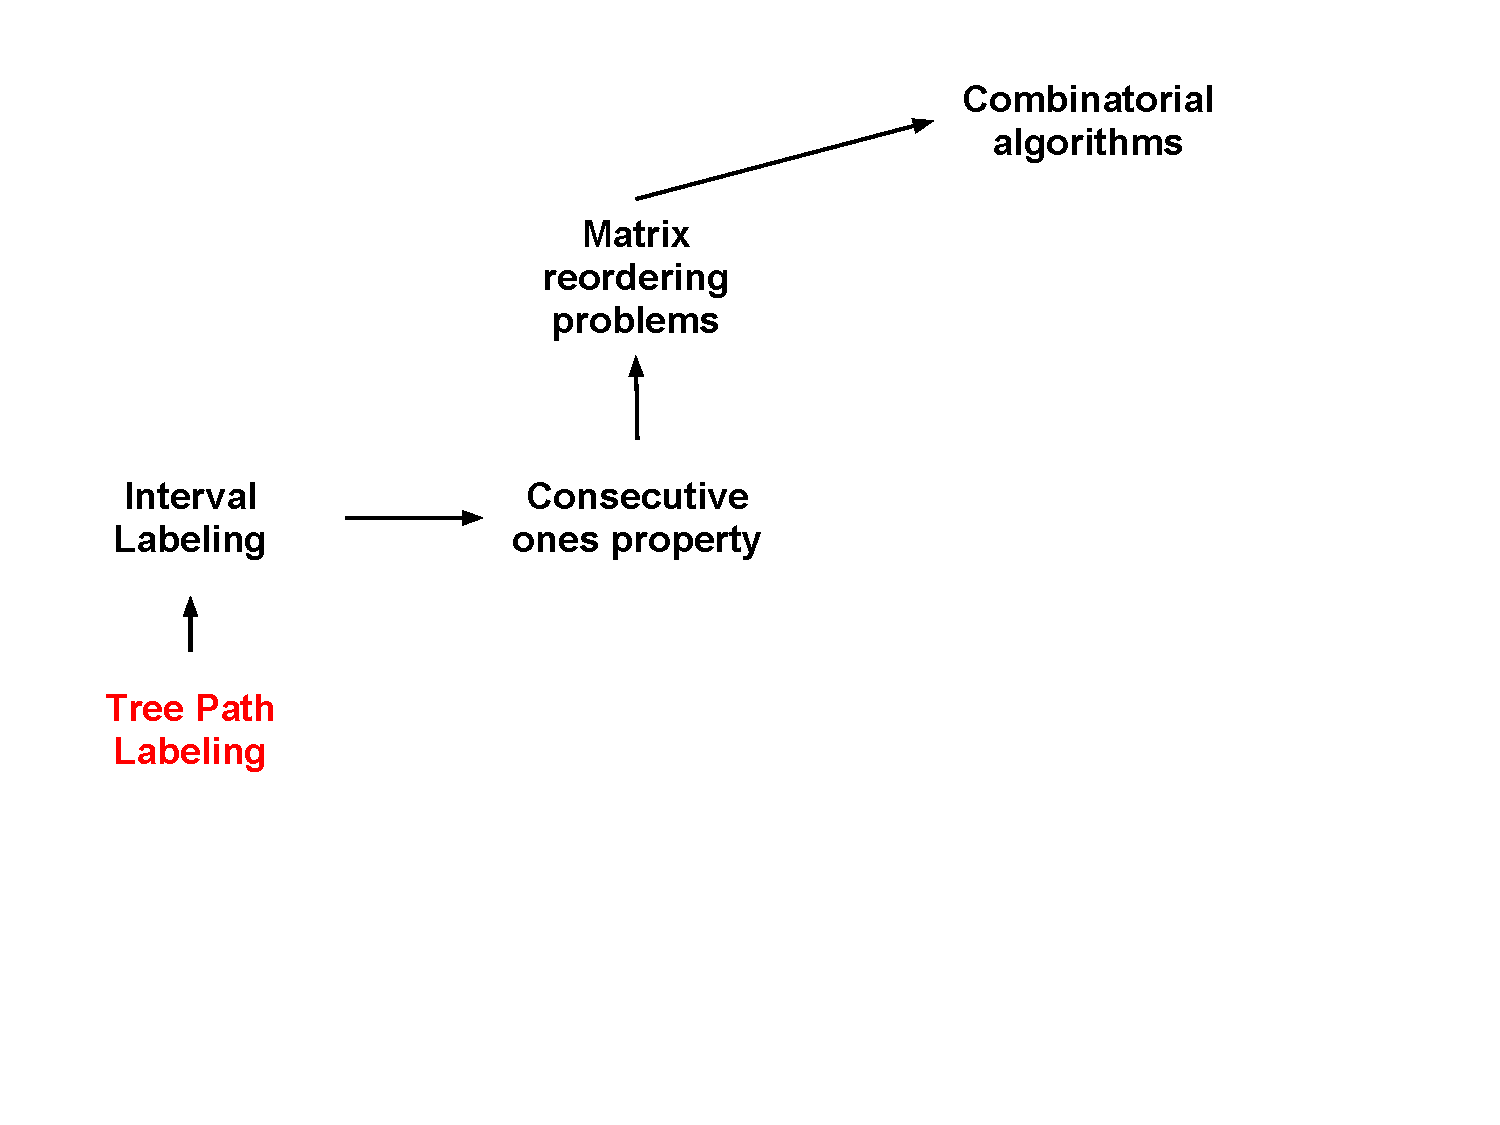
\includegraphics[scale=0.3]{m1.pdf}} 
   \only<2>{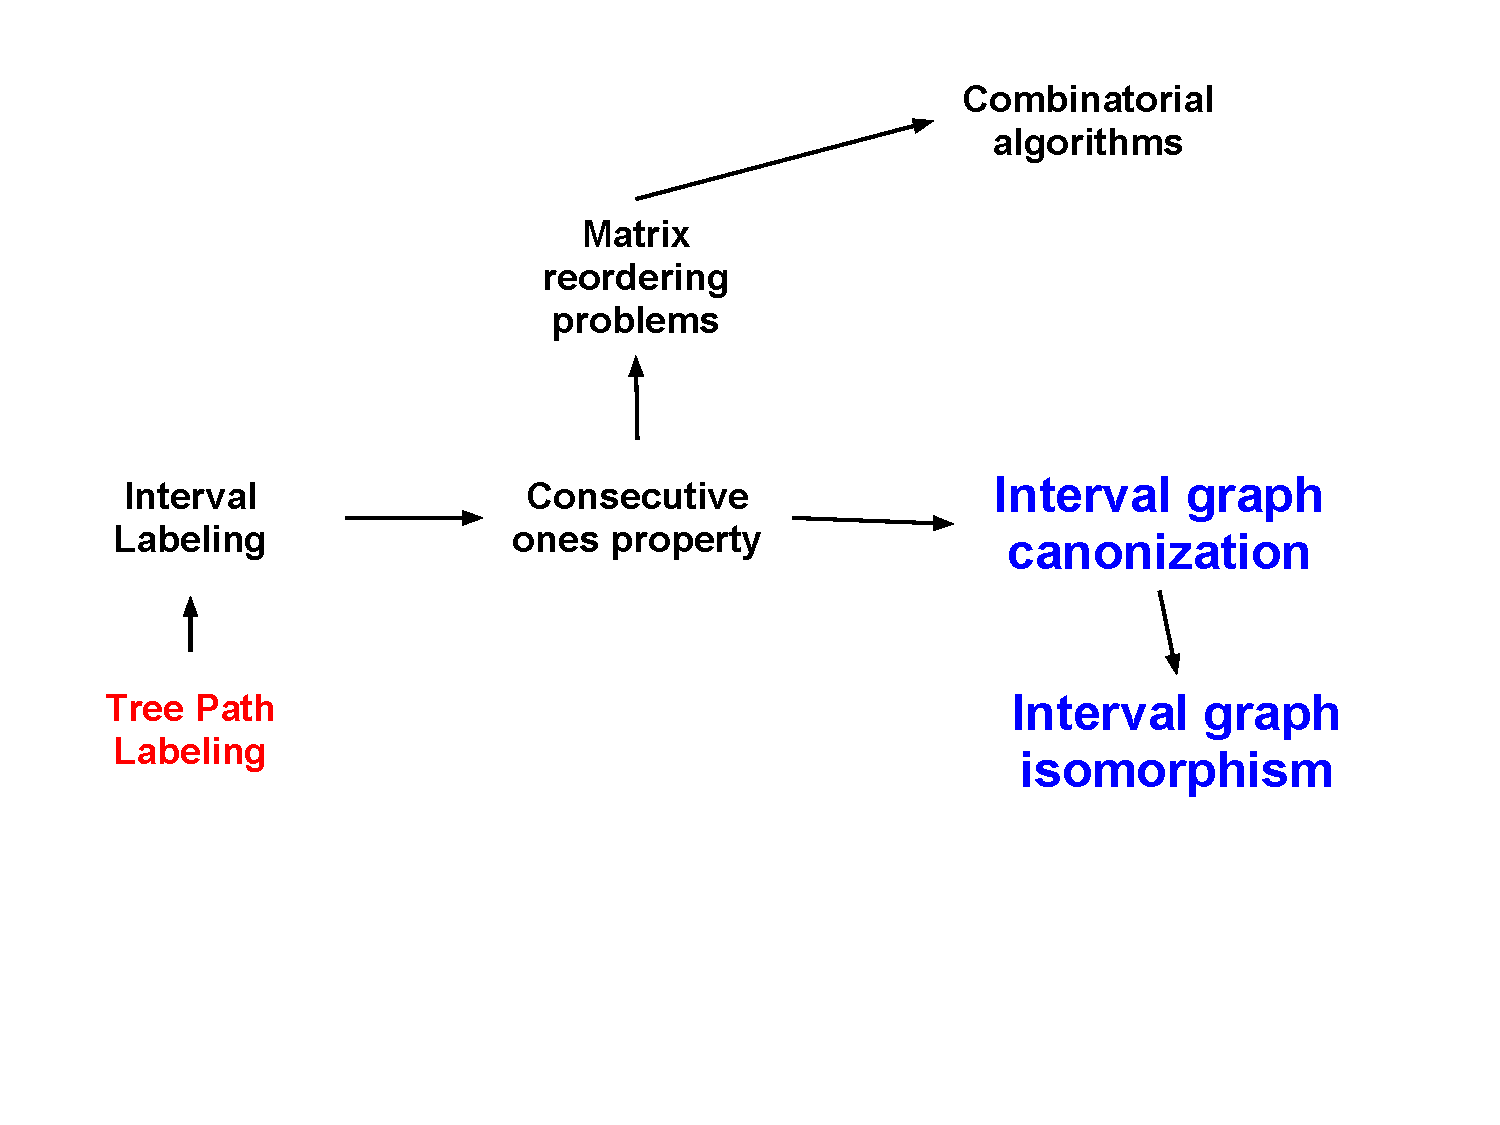
\includegraphics[scale=0.3]{m2.pdf}} 
   \only<3>{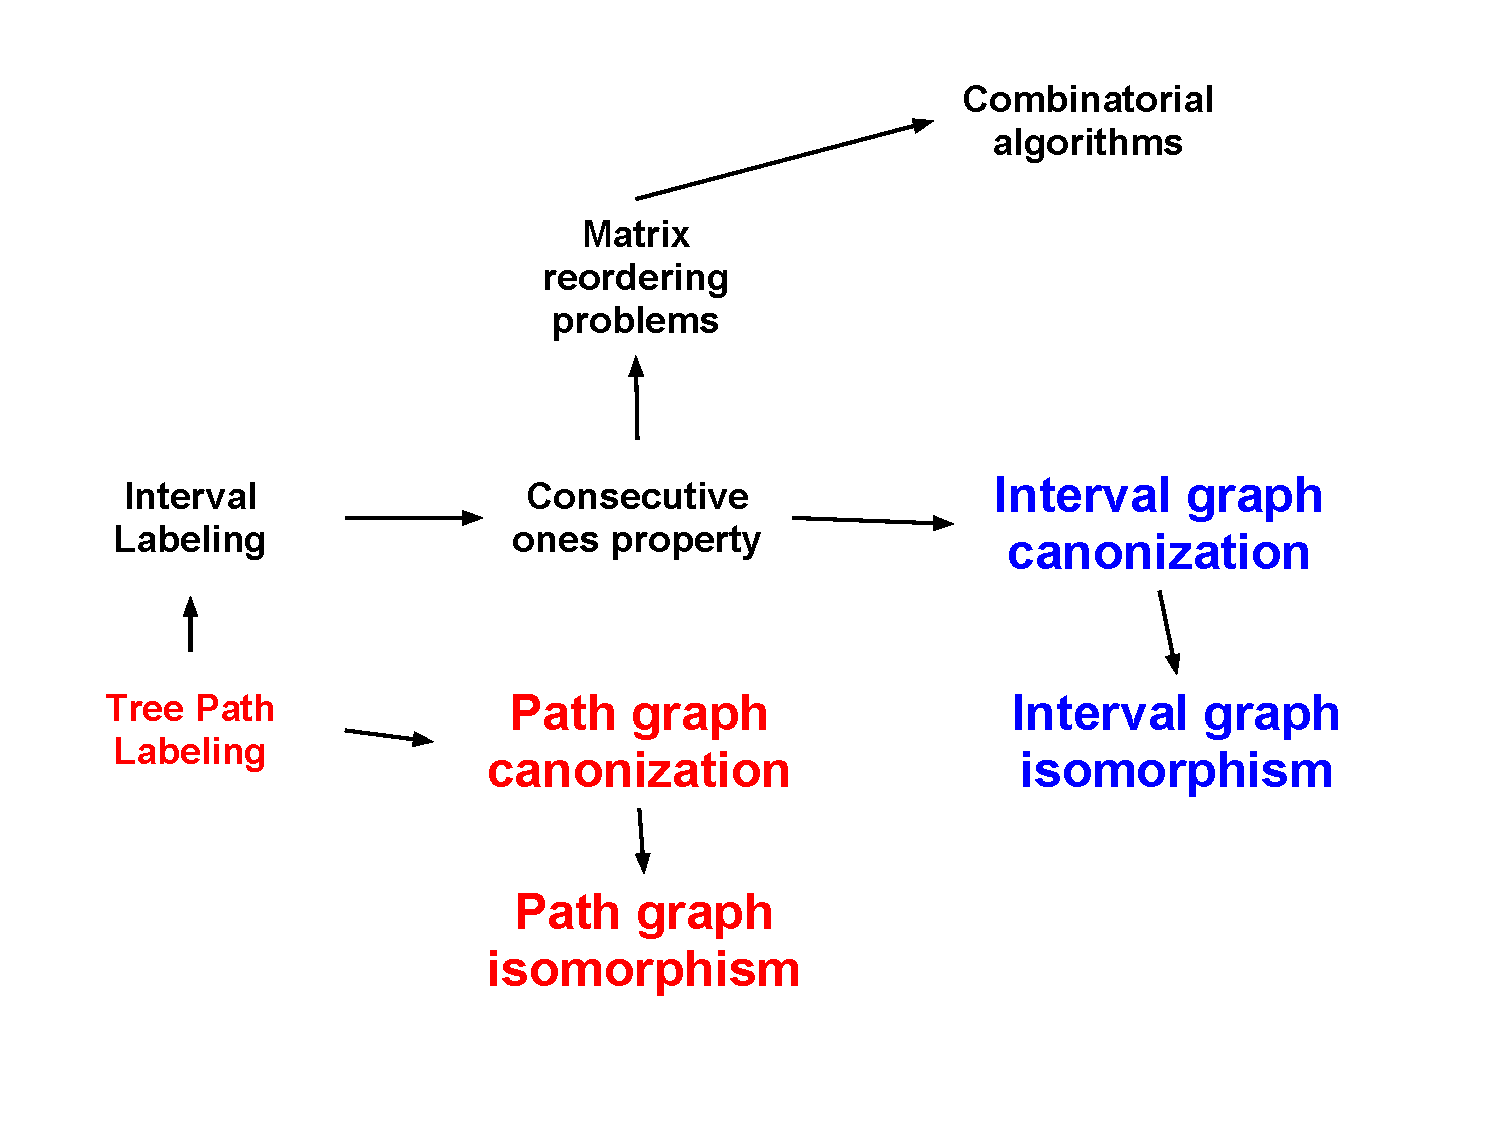
\includegraphics[scale=0.3]{m3.pdf}} 

 \note{}
}

\subsection*{References}
\begin{frame}[allowframebreaks]{References}
  \scriptsize %\footnotesize
  \bibliographystyle{alpha}%
  \bibliography{../lib/cop-variants__thesis}
\end{frame}


\begin{frame}{Thank you}
  Questions?
\end{frame}

% \begin{frame}
% \end{frame} % TEMP: to enforce toc entries when frames haven't been decided
%             % yet.

\end{document}
